En esta sección se presentan las consultas que se utilizaron para experimentar lo propuesto en este trabajo. Las consultas se hicieron sobre dos bases de datos. Una de ellas corresponde a la base de datos de artículos provista por \textit{\textquotedblleft A Data-Driven Journey through Software Engineering Research\textquotedblright}\cite{dataDrive}. La otra base de datos corresponde a atracciones turísticas de Europa. A continuación se describe para cada consulta de cada base da datos la función de similitud, el atributo de complementariedad y el presupuesto. 

\section{Base de datos de artículos}
La base de datos utilizada es la proporcionada por el artículo \textit{\textquotedblleft A Data-Driven Journey through Software Engineering Research\textquotedblright}\cite{dataDrive}. La misma contiene unos $7800$ artículos relacionados con la ingeniería de software presentados en diferentes conferencias entre los años 1975 y 2011 catalogados por autores, tópicos, venues y afiliaciones. Además los artículos están clasificados en tópicos, conocido como \texttt{topicProfile}, que se expresa en porcentajes para cada uno de los tópicos que son tratados. La base considera 38 tópicos para definir el \texttt{topicProfile}. De los $9800$ autores se tiene la información de la universidad a la que pertenecen y de las universidades en que región se encuentran.

El \texttt{topicProfile} es lo que permitirá definir la similitud, no sólo entre los artículos, sino también entre los autores y las universidades de la base de datos de una manera prácticamente directa.

Los criterios de las búsquedas realizadas sobre la base de datos se concibieron a partir de lo que se considera que es de interés general. Por ejemplo, quiénes son los autores que escribieron artículos similares de distintas universidades o las universidades de diferentes regiones donde se escribieron artículos de los mismos tópicos.

Por lo establecido en \cite{compositeRetrival} para las búsquedas se deben realizar las siguientes definiciones:
\begin{itemize}
  \item \textbf{Similitud}: Función que dado dos ítems devuelve la similitud entre estos.
  \item \textbf{Costo}: Función que dado un ítem devuelve el costo del mismo.
  \item \textbf{Presupuesto}: El presupuesto que se tiene, el cual no podrá ser excedido por ningún paquete.
  \item \textbf{Complementariedad}: Propiedad del ítem que es único en cada paquete.
\end{itemize}

Para todas las búsquedas, sin importar el ítem que sea (artículo, autor o universidad), se definió que el costo de cada ítem sea de una unidad y que el presupuesto para cada búsqueda es de cinco unidades. En consecuencia, todos los paquetes de todos los resultados contienen como máximo cinco ítems. Se decidió así para que cada paquete contenga como máximo un número fijo de elementos. Además se decidió que sean diez los paquetes devueltos en cada búsqueda. El motivo para tomar esta decisión es que un humano pueda valorizar el resultado propuesto fácilmente. Entonces, de aquí en adelante, para cada criterio de búsqueda se deben definir únicamente la función de similitud y la propiedad de complementariedad.

Como se mencionó anteriormente, en la base de datos cada artículo cuenta con su \texttt{Topic Profile}. El \texttt{Topic Profile} define el perfil de cada artículo asignándole un porcentaje a cada tópico que se hace referencia. En el caso del artículo \texttt{A Cognitive-Based Mechanism for Constructing Software Inspection Teams} el \texttt{Topic Profile} se compone por los tópicos  REQUIREMENTS, RELIABILITY, TESTING y SOFTWARE QUALITY. El porcentaje de cada uno de estos es 71.43 \%, 17.86 \%, 7.14 \% y 3.57 \% respectivamente.

El modelo computacional del perfil de cada artículo es un vector que la dimensión corresponde a la cantidad de tópicos y cada posición representa un tópico diferente. El valor de cada posición del vector es el porcentaje del tópico que le corresponde a ese artículo según el \textit{Topic Profile} de la base de datos. Más adelante se explica como estos vectores se utilizan para comparar la similitud entre los artículos.

Para los autores no se cuenta con información más allá de los artículos que escribieron, pero sólo con eso alcanza para poder generar un perfil de autores, por lo tanto para cada autor se hace la suma vectorial de cada uno de los \texttt{Topic Profile} de los artículos en los cuales participó y con eso se obtiene el \texttt{Topic Profile de Autores}. Para obtener el perfil de las universidades se aplicó el mismo criterio que para los autores, de hacer la suma vectorial de cada uno de los \texttt{Topic Profile de Autores} pertenecientes a la misma universidad y así generar el \texttt{Topic Profile de Universidades}. En ambos casos se aplica la normalización sobre los vectores resultantes.

Ejemplo de los perfiles de los elementos:
\begin{description}
 \item[Artículo - Topic Profile - Autores]
 \item Artículo 1 - $[$0.20, 0.40, 0.40, 0.00$]$ - Autor 1, Autor 2, Autor 3
 \item Artículo 2 - $[$0.30, 0.70, 0.00, 0.00$]$ - Autor 2, Autor 3
 \item Artículo 3 - $[$0.00, 0.10, 0.00, 0.90$]$ - Autor 2
 \item Artículo 4 - $[$0.00, 0.00, 1.00, 0.00$]$ - Autor 1, Autor 3
\end{description}

\begin{description}
 \item[Autor - Topic Profile - Universidad]
 \item Autor 1 - $[$0.14, 0.27, 0.95, 0.00$]$ - Universidad 1
 \item Autor 2 - $[$0.30, 0.74, 0.25, 0.55$]$ - Universidad 2
 \item Autor 3 - $[$0.27, 0.60, 0.76, 0.0$]$ - Universidad 2
\end{description}

\begin{description}
 \item[Universidad - Topic Profile]
 \item Universidad 1 - $[$0.14, 0.27, 0.95, 0.00$]$
 \item Universidad 2 - $[$0.31, 0.72, 0.54, 0.30$]$
\end{description}

Las consultas realizadas son:
\begin{enumerate}
	\item
		Artículos con tópicos similares presentados en distintas conferencias.
		\begin{itemize}
			\item \textbf{Similitud}: Función que compara el perfil de cada artículo.
			\item \textbf{Complementariedad}: Lugar dónde fue presentado.
		\end{itemize}

	\item
	Autores que escribieron artículos con tópicos similares afiliados en universidades distintas.
	\begin{itemize}
		\item \textbf{Similitud}: Función que compara el perfil de los autores.
		\item \textbf{Complementariedad}: Universidad de pertenencia del autor.
	\end{itemize}

	\item 
	Universidades en las que se escribieron artículos de tópicos similares que se encuentran en distintas regiones. 
	\begin{itemize}
		\item \textbf{Similitud}: Función que compara el perfil de las universidades.
		\item \textbf{Complementariedad}: Región de la institución.
	\end{itemize}
\end {enumerate}

Para obtener resultados de mayor calidad, se depuró de la base de datos aquellos artículos que no contengan la información del autor, de los tópicos (\textbf{topic profile}) o del lugar de publicación (\textbf{venue}). Quedando, luego de la depuración, $5500$ artículos.  

\paragraph{Función de similitud}
La similitud se emplea para comparar dos objetos y determinar qué tan parecido son entre si. En este trabajo la similitud entre los objetos de la base de datos de artículos esta definida por la \textbf{similitud coseno}. Esta es una medida de similitud entre dos vectores en un espacio vectorial provisto de un producto escalar que mide el coseno del ángulo comprendido entre ellos. El coseno para el ángulo cero es 1, es menor a 1 para cualquier otro ángulo y es 0 cuando los vectores son ortogonales. 

Entonces se define la función de similitud $S(V_i, V_j)$ para los vectores $V_i$ y $V_j$ a partir del producto escalar\\

\begin{equation} \label{eq:angulovectorial}
\cos(\theta) =  \dfrac{\overrightarrow{U} . \overrightarrow{V}}{\overrightarrow{\lVert V\lVert}.\overrightarrow{\lVert U\lVert}}
\end{equation}

Para esta instancia los objetos (ahora artículos, autores o universidades) son representados por vectores, donde cada dimensión corresponde a un tópico y el valor se corresponde con el valor del tópico del objeto según la base de datos \cite{dataDrive}. Por lo tanto el objeto $a$ se representa con el vector $V_a = [v_1,v_2,...,v_38]$ que cumple con las siguientes propiedades:
\begin{enumerate}
 \item $v_i \geq 0$
 \item $\sum{v_i} = 1$
\end{enumerate}

Como los componentes de todos los vectores son mayor o igual a cero se obtiene que $0\leq\cos(\theta)\leq1$, que implica que $S(V_i, V_j) \in \left[0, 1\right]$.

\begin{figure}[H]
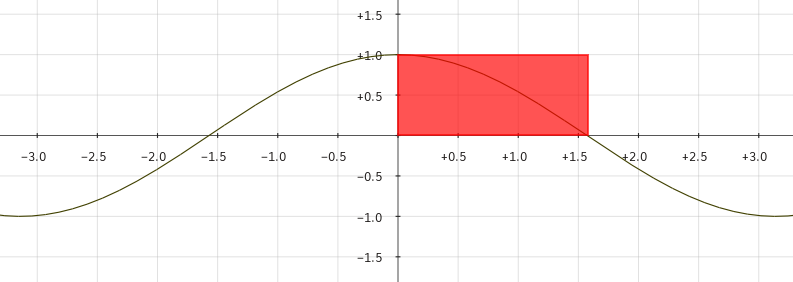
\includegraphics[width=0.8\textwidth]{img/coseno.png}
\caption{Comportamiento de la función $\cos$. En rojo la región que pertenece a la función de similitud}
\label{bus:img-coseno}
\end{figure}

%Para \textbf{similitud coseno} dos vectores proporcionales con la misma dirección la similitud es 1 (ya que es 0 el ángulo que se forma). Por lo que esta similitud no diferencia entre un artículo profesional y un artículo de un diario que cubre el mismo tópico. Por ejemplo si dos artículos que cubren un mismo y único tópico, pero para uno el valor del tópic Esta debilidad de la medida basada en el ángulo no interfiere en este trabajo por la segunda propiedad de los vectores del problema, porque para que dos vectores sean proporcionalmente iguales tienen que ser idénticos y en tal caso es correcto que la similitud entre ellos sea 1.

El cálculo de similitud de los artículos, autores y universidades se realizó previamente a la ejecución de los algoritmos de búsquedas. El motivo por el cual se decidió hacer de esta manera fue para simplificar la ejecución ya que el costo de calcular el $\cos(\theta)$ de los vectores es alto.

\section{Atracciones turísticas}
Se utilizó una instancia de datos correspondiente a 200 atracciones turísticas de Europa, con datos relevados del sitio \textit{TripAdvisor}. De cada atracción se tiene la información del precio, del tipo (parque, museo, edificio) y de la distancia geográfica con el resto de las atracciones.

El propósito de la búsqueda es darle al usuario distintas opciones de circuitos turísticos, en el cual las atracciones de cada circuito se encuentran geográficamente cerca para evitar realizar largos traslados; de distinto tipo para que haya más variedad y que que todo el circuito este acotado al presupuesto del turista. Por lo tanto el modelo de la búsqueda quedo diseñada de la siguiente manera:

\begin{itemize}
	\item \textbf{Similitud}: La inversa de la distancia entre las atracciones. 
	\item \textbf{Costo}: Precio de la atracción. 
	\item \textbf{Presupuesto}: Presupuesto del turista. 
	\item \textbf{Complementariedad}: Tipo de atracción.
\end{itemize}